\documentclass[conference]{IEEEtran}
\IEEEoverridecommandlockouts
\usepackage{cite}
\usepackage{amsmath,amssymb,amsfonts}
\usepackage{algorithmic}
\usepackage{graphicx}
\usepackage{textcomp}
\usepackage{booktabs}
\usepackage{multirow}
\usepackage{url}
\usepackage{hyperref}
\usepackage{tikz}
\usetikzlibrary{positioning,arrows.meta,calc,fit,backgrounds}

\def\BibTeX{{\rm B\kern-.05em{\sc i\kern-.025em b}\kern-.08em
    T\kern-.1667em\lower.7ex\hbox{E}\kern-.125emX}}

% NOTE ON COMPILING: the bibliography below is a plain `thebibliography`
% environment (no .bib file, no bibtex/biber run required). \cite{...}
% commands resolve against \bibitem labels via the .aux file, which means
% a SINGLE pdflatex pass will show unresolved "[?]" citation marks even
% though the source is correct. Compile twice in a row:
%   pdflatex deepfake_detection_ieee.tex
%   pdflatex deepfake_detection_ieee.tex
% (a third pass is only needed if page/section cross-references shift).

\begin{document}

\title{Multi-Modal Deepfake Detection with Frozen Self-Supervised Backbones,\\
Cross-Region Attention, and Adaptive Gated Fusion:\\
A Systematic Cross-Dataset Generalization Study}

% NOTE: fill in the placeholders below with your real name/affiliation.
% IMPORTANT: do not wrap the replacement text in square brackets ([ ]) --
% literal "[" characters inside \IEEEauthorblockN/A break IEEEtran's
% internal \maketitle parsing ("Missing number, treated as zero" error).
\author{
\IEEEauthorblockN{Abhijith Reddy Chalamalla}
\IEEEauthorblockA{\textit{Department of Computer Science and Engineering} \\
\textit{Amrita School of Computing}\\
Coimbatore, India \\
ch.sc.u4cse23204@REPLACE-WITH-FULL-DOMAIN}
}

\maketitle

\begin{abstract}
Deepfake detectors routinely report near-perfect accuracy on their own
benchmark's held-out test split, yet the practical value of such a system
depends on whether its performance survives exposure to previously unseen
generation methods. We present a two-stage, dual-modality deepfake
detection system that combines frozen self-supervised visual and audio
backbones (DINOv2 ViT-S/14 and Whisper-tiny), a four-region
(face/eyes/lips/jaw) cross-region attention module, per-modality bidirectional
LSTMs, a two-layer fusion Transformer, and a Gated Multimodal Unit (GMU) for
adaptive visual-audio weighting, together with a low-rank adaptation (LoRA)
fine-tuning stage and an auxiliary multi-class forgery-type head. Trained on
a pool of 44{,}561 videos from FakeAVCeleb, PolyGlotFake, FaceForensics++,
and Celeb-DF-v2 (the latter was previously mislabeled as FaceForensics++ in
this pipeline; both this and a separate identity-leakage bug in the
train/val/test splitting logic were found and fixed as part of this work,
Section~IV-A), the system reaches AUC~0.998 and $>$98\% accuracy
in-distribution -- verified by retraining \emph{both} of our two candidate
Stage B recipes against the corrected, genuinely identity-disjoint split and
re-selecting canonical by validation AUC exactly as our own methodology
requires (Section~IV-A), rather than reporting an unverified number: the
selected recipe is unchanged from before the fix, in-distribution AUC was
essentially unaffected by the leakage bug (0.9962$\to$0.9984 for this
recipe), and DFDC cross-dataset AUC under the corrected split (0.7091) is
in line with our original finding (0.71). Critically, we reserve
the DeepFake Detection Challenge (DFDC) dataset entirely for
out-of-distribution evaluation, excluded from every stage of training,
validation, and threshold selection. Critically, DFDC is also excluded from
\emph{configuration selection}: the deployed configuration is chosen using
validation AUC alone, and DFDC results for all five candidate Stage B
configurations are then reported as a single blind post-hoc evaluation,
rather than retrospectively reporting whichever configuration happened to
score best on DFDC. On this genuinely unseen distribution, AUC ranges from
0.65--0.71 across five Stage B configurations and one Stage A prerequisite
baseline (frozen-backbone baseline, LoRA fine-tuning, data augmentation,
weight decay, Self-Blended Images synthetic data, and an SRM
frequency-domain branch), none of which closes more than a fraction of the
gap. We complement the ablation
with quantitative error analysis, a modified Grad-CAM/attention-rollout
explainability pipeline, and a causal boundary-cue masking experiment; the
latter contradicts the boundary-reliance hypothesis the Grad-CAM
visualization initially suggested, illustrating that attention-map-based
diagnosis requires quantitative verification rather than acceptance at face
value. We report this observed
generalization limit as a primary finding rather than obscuring it behind
in-distribution numbers, and argue that closing it requires training-data
diversity across
generation-method families rather than further architectural or
regularization tuning on the same three datasets.
\end{abstract}

\begin{IEEEkeywords}
deepfake detection, multi-modal learning, self-supervised learning, DINOv2,
Whisper, low-rank adaptation, gated multimodal unit, cross-dataset
generalization, explainable AI, Grad-CAM
\end{IEEEkeywords}

\section{Introduction}

The proliferation of generative adversarial networks (GANs), autoencoder
face-swap pipelines, and diffusion-based synthesis tools has made
photorealistic facial forgery -- \textit{deepfakes} -- inexpensive to produce
and increasingly difficult to detect by eye \cite{tolosana2020survey}. The
resulting risks to information integrity, identity security, and public
trust in audiovisual media have driven a large body of detector research,
almost all of which is evaluated on the same handful of public benchmarks
\cite{rossler2019faceforensics, dolhansky2020dfdc, khalid2021fakeavceleb}.

A persistent, under-reported problem in this literature is that
\textit{in-distribution} accuracy -- performance on a held-out split of the
\emph{same} dataset(s) used for training -- is a poor proxy for real-world
usefulness. Detectors learn to recognize the specific compression artifacts,
generator fingerprints, and post-processing signatures of the generation
pipelines present in their training data, and that signal frequently fails
to transfer to a video produced by a different, unseen generation method
\cite{tolosana2020survey, wang2020cnn, cozzolino2018forensictransfer}. A
detector that reports 99\% accuracy on its own benchmark but silently
degrades to substantially degraded performance on a forgery technique it has not seen
cannot be considered solved in a deployment setting.

This paper makes two contributions. First, we describe a complete
multi-modal deepfake detection architecture built around frozen
self-supervised visual (DINOv2 \cite{oquab2023dinov2}) and audio (Whisper
\cite{radford2023whisper}) backbones, fine-tuned efficiently with low-rank
adaptation (LoRA) \cite{hu2022lora}, and fused adaptively across modalities
with a Gated Multimodal Unit (GMU) \cite{arevalo2017gmu}. The architecture
additionally uses region-level cross-attention across four facial regions,
bidirectional LSTM temporal modeling, an auxiliary multi-class
manipulation-type head, and an explainability pipeline that combines a
DINOv2-specific adaptation of Grad-CAM \cite{selvaraju2017gradcam} with
Transformer attention rollout \cite{abnar2020rollout}.

Second, and more centrally, we treat cross-dataset generalization as a
first-class experimental question rather than an afterthought. We reserve
the DFDC dataset \cite{dolhansky2020dfdc} in its entirety -- never touched
during training, validation, decision-threshold selection, or, critically,
\emph{configuration selection} (Section~V-C) -- as a probe of genuine
out-of-distribution performance, and report six independent
attempts to close the resulting in-distribution/cross-dataset gap:
frozen-backbone extraction, LoRA fine-tuning, data augmentation, weight
decay regularization, Self-Blended Images (SBI) synthetic
data~\cite{shiohara2022sbi}, and a hand-engineered SRM frequency-domain
branch~\cite{fridrich2012srm}. We report the outcome of every attempt,
including interventions that yielded no improvement or reduced
performance, together with a
quantitative error analysis and an explainability-driven diagnosis of
\emph{why} the gap persists. We believe this transparency -- reporting the
observed 0.71 AUC generalization limit rather than only the 0.996
in-distribution headline number -- is itself a useful empirical
contribution, consistent
with the community's growing recognition that cross-dataset evaluation, not
in-dataset evaluation, is the meaningful test of a deepfake detector
\cite{tolosana2020survey, haliassos2021lipforensics, cao2022recce}.

The remainder of this paper is organized as follows. Section~II reviews
related work. Section~III describes the proposed architecture. Section~IV
details the datasets, splitting protocol, and training procedure. Section~V
presents in-distribution and cross-dataset results, the six-attempt
generalization ablation, and the diagnostic analysis. Section~VI discusses
implications and limitations. Section~VII concludes.

\section{Related Work}

\subsection{Spatial and Frequency-Domain Detectors}
Early deepfake detectors treated the problem as binary image classification,
using CNN backbones such as Xception \cite{chollet2017xception} or compact
purpose-built networks such as MesoNet \cite{afchar2018mesonet} to pick up
mesoscopic blending artifacts. FaceForensics++ \cite{rossler2019faceforensics}
established the standard evaluation protocol for this line of work.
Frequency-domain approaches complement spatial CNNs by exposing GAN
up-sampling artifacts that are less visible in the spatial domain; SRM-style
high-pass residual filters, originally developed for steganalysis
\cite{fridrich2012srm}, are a common hand-engineered choice for this
purpose, and learned frequency-aware branches such as F3-Net
\cite{qian2020f3net} extend the idea to end-to-end training. A related line
of work targets the generic blending boundary left by any face-compositing
operation rather than a specific generator's fingerprint, exemplified by
Face X-Ray \cite{li2020facexray}; our Self-Blended Images attempt
(Section~V-C) is built on this boundary-artifact framing, and our
Grad-CAM spot-check (Section~V-D) initially appeared to connect to it as
well, though a subsequent causal ablation (also Section~V-D) did not bear
that reading out.

\subsection{Temporal and Multi-Modal Detectors}
Because many forgeries are frame-consistent but temporally or
cross-modally inconsistent, later work incorporates recurrent or attention-based
temporal modeling (LSTMs \cite{hochreiter1997lstm,schuster1997bidirectional},
Transformers \cite{vaswani2017attention}) and audio-visual synchronization
cues, as in LipForensics \cite{haliassos2021lipforensics} and FTCN
\cite{zheng2021ftcn}, both of which report substantially better
cross-manipulation generalization than purely spatial detectors. The DFDC
\cite{dolhansky2020dfdc} and FakeAVCeleb
\cite{khalid2021fakeavceleb} datasets were released specifically to support
multi-modal and cross-manipulation-method evaluation; PolyGlotFake extends
this to multilingual audio-driven forgeries \cite{polyglotfake2025}.
Gated Multimodal Units \cite{arevalo2017gmu} provide a principled,
learned mechanism for weighting unreliable or missing modalities, which we
adopt for visual-audio fusion.

\subsection{Self-Supervised Backbones and Parameter-Efficient Fine-Tuning}
Self-supervised vision backbones such as DINOv2 \cite{oquab2023dinov2} and
speech backbones such as Whisper \cite{radford2023whisper} are trained on
web-scale unlabeled or weakly-labeled data and produce general-purpose
representations that transfer well across downstream tasks. Because full
fine-tuning of such backbones on a comparatively small forgery dataset risks
catastrophic overfitting to dataset-specific artifacts, we use Low-Rank
Adaptation (LoRA) \cite{hu2022lora}, which freezes the backbone and injects
small trainable low-rank update matrices into a subset of layers.

\subsection{Synthetic Data for Generalization}
Self-Blended Images (SBI) \cite{shiohara2022sbi} synthesize pseudo-forgeries
from real images alone, by blending a warped, color-jittered copy of a face
back onto itself, with the goal of teaching a generic
``blending-boundary'' cue that is not tied to any specific generator's
fingerprint. We include SBI as one of our six generalization-improvement
attempts.

\subsection{Explainability}
Grad-CAM \cite{selvaraju2017gradcam} was designed for convolutional
architectures and does not transfer directly to Vision Transformers that
pool only a CLS token, since patch tokens frequently have no differentiable
path to the classification logit. Attention rollout \cite{abnar2020rollout}
addresses a related problem for Transformer stacks by recursively composing
per-layer attention matrices (with an identity term for the residual
connection) into a single input-attribution map. We combine an
architecture-specific Grad-CAM adaptation for DINOv2 with attention rollout
over our fusion Transformer, described in Section~III-I.

\section{Proposed Architecture}

\begin{figure*}[t]
\centering
\resizebox{\textwidth}{!}{%
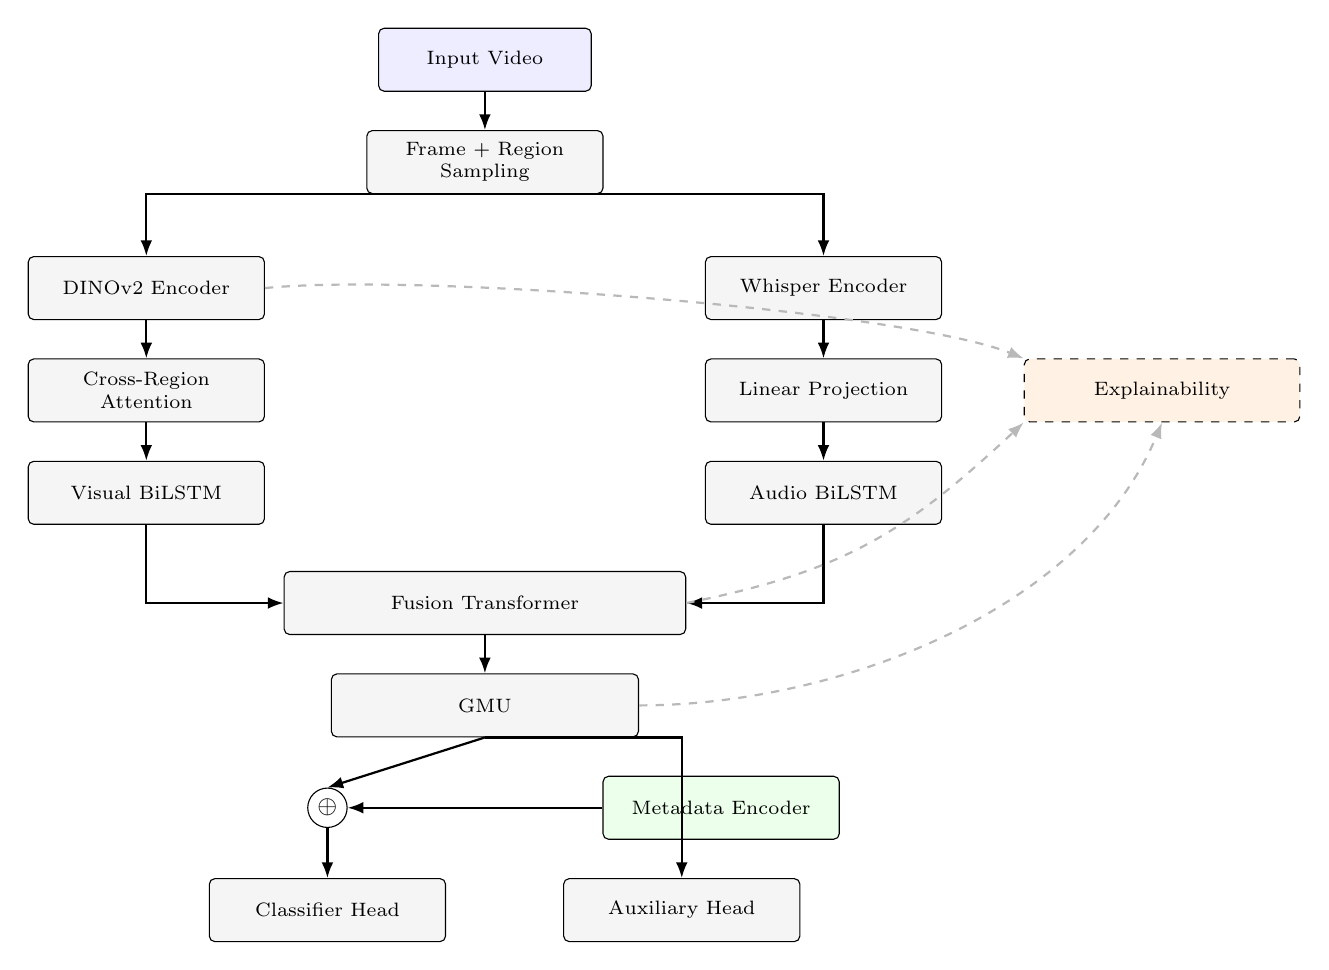
\begin{tikzpicture}[
    font=\scriptsize,
    blk/.style={rectangle, draw, rounded corners=2pt, align=center,
      minimum height=8mm, text width=27mm, fill=gray!8, inner sep=1.5mm},
    io/.style={blk, fill=blue!7, text width=24mm},
    metablk/.style={blk, fill=green!8, text width=27mm},
    expl/.style={blk, dashed, fill=orange!10, text width=32mm},
    circ/.style={circle, draw, minimum size=5mm, inner sep=0pt, font=\small},
    arr/.style={-{Latex[length=2mm]}, thick},
    darr/.style={-{Latex[length=2mm]}, dashed, gray!55, thick}
  ]

  \node[io]  (video)   at (0,0)        {Input Video};
  \node[blk] (sample)  at (0,-1.3)     {Frame + Region\\Sampling};

  \node[blk] (dino)    at (-4.3,-2.9)  {DINOv2 Encoder};
  \node[blk] (cra)     at (-4.3,-4.2)  {Cross-Region\\Attention};
  \node[blk] (vlstm)   at (-4.3,-5.5)  {Visual BiLSTM};

  \node[blk] (whisper) at (4.3,-2.9)   {Whisper Encoder};
  \node[blk] (aproj)   at (4.3,-4.2)   {Linear Projection};
  \node[blk] (alstm)   at (4.3,-5.5)   {Audio BiLSTM};

  \node[blk, text width=48mm] (fusion) at (0,-6.9) {Fusion Transformer};
  \node[blk, text width=36mm] (gmu)    at (0,-8.2) {GMU};

  \node[circ]     (plus) at (-2.0,-9.5)  {$\oplus$};
  \node[metablk]  (meta) at (3.0,-9.5)   {Metadata Encoder};
  \node[blk]      (clf)  at (-2.0,-10.8) {Classifier Head};
  \node[blk]      (aux)  at (2.5,-10.8)  {Auxiliary Head};

  \node[expl] (explain) at (8.6,-4.2) {Explainability};

  \draw[arr] (video) -- (sample);
  \draw[arr] (sample.south) -| (dino.north);
  \draw[arr] (sample.south) -| (whisper.north);
  \draw[arr] (dino) -- (cra);
  \draw[arr] (cra) -- (vlstm);
  \draw[arr] (whisper) -- (aproj);
  \draw[arr] (aproj) -- (alstm);
  \draw[arr] (vlstm.south) |- (fusion.west);
  \draw[arr] (alstm.south) |- (fusion.east);
  \draw[arr] (fusion) -- (gmu);
  \draw[arr] (gmu.south) -- (plus.north);
  \draw[arr] (meta.west) -- (plus.east);
  \draw[arr] (plus.south) -- (clf.north);
  \draw[arr] (gmu.south) -| (aux.north);

  \draw[darr] (dino.east) .. controls +(20mm,2mm) and +(-15mm,6mm) .. (explain.north west);
  \draw[darr] (fusion.east) .. controls +(20mm,4mm) and +(-15mm,-14mm) .. (explain.south west);
  \draw[darr] (gmu.east) .. controls +(25mm,0mm) and +(-10mm,-24mm) .. (explain.south);
\end{tikzpicture}%
}
\caption{End-to-end architecture (implementation detail omitted from the
diagram for readability is given here). Frame + Region Sampling: 8
uniformly-sampled frames, 4 region crops per frame (face / eyes / lips /
jaw). DINOv2 / Whisper Encoders: DINOv2 ViT-S/14 and Whisper-tiny, both
frozen in Stage A and partially re-opened via LoRA adapters in Stage B (the
same backbone stack is used at both stages; Stage A caches frozen features,
Stage B trains end-to-end on raw crops). Cross-Region Attention: a
region-projection layer followed by multi-head self-attention across the 4
region tokens per frame (Section~III-D). Fusion Transformer: 2 layers, 4
heads, with learned modality embeddings distinguishing visual from audio
tokens (Section~III-F). GMU: the Gated Multimodal Unit that adaptively
weights the pooled visual and audio streams (Section~III-F). Metadata
Encoder: a small MLP over the 34-dimensional \texttt{ffprobe}-derived
feature vector (Section~III-G). The $\oplus$ node denotes concatenation of
the GMU's fused representation with the metadata embedding, which feeds
only the Classifier Head (real/fake logit); the Auxiliary Head (9-way
manipulation-type classification) reads the fused representation directly,
without metadata. Dashed arrows/box indicate the explainability pathway
(Section~III-I) -- Grad-CAM over DINOv2's CLS-to-patch attention, attention
rollout over the fusion Transformer, and the GMU gate value -- which
consumes intermediate model state but does not feed back into the
classifier.}
\label{fig:architecture}
\end{figure*}

Figure~\ref{fig:architecture} summarizes the pipeline. The system consumes a
video and produces (i) a real/fake probability, (ii) an auxiliary
manipulation-type distribution, and (iii) a GMU gate value indicating the
relative contribution of the visual and audio streams.

\subsection{Frame and Region Sampling}
Eight frames per video are selected by uniform temporal index sampling,
\begin{equation}
t_i = \left\lfloor \frac{iN}{8} \right\rfloor, \quad i \in \{0,1,\dots,7\},
\end{equation}
given $N$ total frames, so that the sample spans the full video rather than
only its opening seconds. The frame count was set, together with the batch-size and
gradient-accumulation choices of Section~IV-B, to fit within the 8~GB GPU
memory budget available for this project; we did not run a systematic
ablation over the frame count, so denser sampling (e.g., 16 or 32 frames)
remains an open direction rather than a value we can claim is optimal.
Faces are localized with MediaPipe Face Landmarker \cite{lugaresi2019mediapipe} (468
landmarks, minimum detection confidence 0.4), with MTCNN \cite{zhang2016mtcnn} as a coarse-bounding-box
fallback and the full frame as a last resort when neither detector fires.
From the resulting face bounding box $(x_1,y_1,x_2,y_2)$ with height
$f_h = y_2 - y_1$, four regions are cropped and resized to $224{\times}224$:
\textit{face} (the full box), \textit{eyes} (top 40\% of box height),
\textit{lips} (bottom 40\%), and \textit{jaw} (from 75\% down to 15\% below
the box, chosen because face-swap blending seams concentrate around the
jawline-to-neck boundary). These four regions, rather than e.g. the
forehead or cheeks, were chosen because prior forgery-detection work
consistently localizes artifacts to facial boundaries and blending seams
\cite{li2020facexray}, the periocular region (blink-rate and gaze
anomalies), and the lips (audio-visual synchronization
\cite{haliassos2021lipforensics}).

\subsection{Visual Feature Extraction: DINOv2}
Each of the four $224{\times}224$ region crops, for each of the eight
frames, is encoded independently by DINOv2 ViT-S/14
\cite{oquab2023dinov2}, a self-supervised Vision Transformer
\cite{dosovitskiy2021vit} trained with a
student-teacher distillation objective on large-scale curated image data.
We retain only the 384-dimensional CLS token per region per frame, giving a
visual feature tensor of shape $(8, 4, 384)$ per video. DINOv2 is chosen
over a supervised ImageNet backbone because its self-supervised objective
encourages representations of generic visual structure rather than
class-discriminative shortcuts, which is desirable when the discriminative
task at hand (forgery detection) is not the task the backbone was trained
for. The ViT-S/14 variant specifically was selected, over the larger
ViT-B/14 or ViT-L/14 variants, to fit the project's 8~GB GPU memory budget
(Section~IV-B); we did not run a comparative ablation against the larger
DINOv2 variants, so we cannot claim ViT-S/14 is optimal, only that it is
the variant this budget supported.

\subsection{Audio Feature Extraction: Whisper}
The audio track is encoded with the Whisper-tiny encoder
\cite{radford2023whisper}, a Transformer speech encoder trained via
large-scale weakly-supervised multitask learning. Whisper-tiny (39M
parameters), the smallest variant in the Whisper family, was likewise
selected to fit the same 8~GB memory budget as the visual backbone; larger
Whisper variants (base, small, and above) were not evaluated in this
project. Whisper's encoder emits a
fixed 1500-step sequence (from its 30-second-padded input convention),
which is adaptively average-pooled (\texttt{adaptive\_avg\_pool1d}) down to
8 temporal steps to align exactly with the 8 visual frames -- a design
choice that lets the fusion Transformer (Section~III-F) attend across
modalities token-for-token without any additional interpolation or
asynchronous token-matching step, at the cost of discarding whatever
finer-grained temporal audio structure exists within each of the 8
pooled windows. This produces an audio feature tensor of shape $(8, 384)$.

\subsection{Cross-Region Attention}
The four per-frame region embeddings are first linearly projected from 384
to the model's working dimension $d=256$. A learned per-region embedding is
added (so the attention layer can distinguish face/eyes/lips/jaw
identity), and a standard multi-head self-attention layer (4 heads) lets
the four regions attend to each other within each frame:
\begin{equation}
\mathbf{a}_t = \mathrm{LayerNorm}\big(\mathrm{MHA}(\mathbf{r}_t,\mathbf{r}_t,\mathbf{r}_t) + \mathbf{r}_t\big),
\end{equation}
where $\mathbf{r}_t \in \mathbb{R}^{4\times d}$ are the four region tokens
at frame $t$ (with region embeddings added), $\mathrm{MHA}(\cdot)$ denotes
standard multi-head self-attention, and $\mathrm{LayerNorm}(\cdot)$ denotes
layer normalization. The four attended region
vectors are then mean-pooled to a single per-frame vector, so that, e.g., an
inconsistency localized to the lips can influence the representation of the
whole face region and vice versa.

\subsection{Temporal Modeling}
The per-frame fused region vector is passed through a single-layer
bidirectional LSTM \cite{hochreiter1997lstm,schuster1997bidirectional}
(hidden size 128 per direction, concatenated to $d=256$) to capture
frame-to-frame dynamics such as unnatural blinking or micro-expression
discontinuities. The audio branch is treated symmetrically: the projected
384$\to$256 Whisper features pass through their own single-layer BiLSTM. We
deliberately use a single BiLSTM layer per branch rather than a deeper
stack, since a two-layer BiLSTM was found to overfit given the size of the
training data.

\subsection{Fusion Transformer and Gated Multimodal Unit}
Learned modality embeddings are added to the visual and audio token
sequences, which are then concatenated along the time axis (16 tokens
total: 8 visual + 8 audio) and passed through a two-layer Transformer
encoder (4 heads, feedforward dimension 512, dropout 0.2)
\cite{vaswani2017attention}, allowing every visual frame to attend to every
audio frame and vice versa. The fused visual and audio token streams are
then separately mean-pooled back to single vectors $\mathbf{v},\mathbf{a}
\in \mathbb{R}^{256}$, and combined with a Gated Multimodal Unit
\cite{arevalo2017gmu}:
\begin{align}
z &= \sigma\big(W_g[\mathbf{v};\mathbf{a}] + b_g\big), \\
\mathbf{f} &= z \odot \mathbf{v} + (1-z) \odot \mathbf{a},
\end{align}
where $W_g$ and $b_g$ are learnable gating parameters, $\sigma(\cdot)$ is
the sigmoid function, and $\odot$ denotes element-wise multiplication; $z
\in (0,1)^{256}$ is the resulting element-wise gate. Its mean over dimensions
gives a single interpretable scalar in $[0,1]$ (1 = fully visual, 0 = fully
audio) reported alongside every prediction, letting the system communicate
\emph{which modality it relied on} for a given decision, rather than
returning a single opaque probability.

\subsection{Metadata, Classification, and Auxiliary Heads}
A 34-dimensional container/codec feature vector -- derived via FFmpeg's
\texttt{ffprobe} utility and comprising 13 normalized numeric fields (file
size, duration, resolution, frame rate, bitrates, sample rate, channel
count, Group of Pictures (GOP) length, frame count, rotation), one-hot
video codec (5), audio codec (5),
pixel format (3), and container type (3), plus 5 boolean flags (variable
frame rate, missing streams, etc.) -- is embedded through a small MLP
(34$\to$32, ReLU) and concatenated with the fused representation
$\mathbf{f}$. A classifier head (Linear(288,128)$\to$ReLU$\to$Dropout(0.3)
$\to$Linear(128,1)) produces the real/fake logit. In parallel, an
auxiliary linear head predicts one of 9 manipulation-type classes (real,
faceswap, faceswap-wav2lip, fsgan, fsgan-wav2lip, rtvc, wav2lip,
video\_retalking, unknown\_fake -- a taxonomy unified across FakeAVCeleb's
method labels and PolyGlotFake's sync-technique labels) directly from
$\mathbf{f}$, which acts as an auxiliary loss that pushes the shared
representation to be sensitive to \emph{which kind} of artifact is present,
not only to the binary real/fake decision.

\subsection{Two-Stage Training: Frozen Backbone, then LoRA}
Training proceeds in two stages. \textbf{Stage A} freezes DINOv2 and
Whisper entirely and caches their outputs to disk, training only the
region/audio projections, cross-region attention, BiLSTMs, fusion
Transformer, GMU, and classification/auxiliary heads. \textbf{Stage B}
re-opens a small number of backbone layers via LoRA \cite{hu2022lora},
using the PEFT library: for DINOv2, LoRA adapters (rank $r=8$,
$\alpha=16$, dropout 0.1) are injected into the attention QKV/output
projections and both MLP layers of the last 4 of 12 ViT blocks; for
Whisper's encoder, the same LoRA configuration is injected into the last 1
of 4 encoder blocks. This targets the layers most likely to encode
task-relevant, rather than purely general-purpose, visual/acoustic
structure, while leaving the bulk of each pretrained backbone untouched --
a deliberate compromise between adapting to the forgery-detection task and
preserving the backbones' generic representational quality (relevant to the
generalization question in Section~V).

\subsection{Explainability: Grad-CAM Adaptation and Attention Rollout}
Standard Grad-CAM \cite{selvaraju2017gradcam} cannot be applied to DINOv2's
patch tokens as-is: in DINOv2's \texttt{forward\_features}, the CLS token
and patch tokens are sibling slices of the same normalized output, and only
the CLS token is consumed downstream by the visual branch, so patch tokens
have no differentiable path to the logit -- their gradient is identically
\texttt{None} regardless of correct \texttt{retain\_grad()} usage. We
resolve this by manually replaying the last DINOv2 Transformer block with
an explicit, non-fused softmax attention computation (rather than
\texttt{scaled\_dot\_product\_attention}), which exposes a real,
differentiable CLS-to-patch attention row that \emph{is} on the gradient
path (the CLS output is literally an attention-weighted sum of patch
values). Grad-CAM's weight$\times$activation formulation is then applied to
that attention row instead of to patch activations directly. Separately, we
apply attention rollout \cite{abnar2020rollout} across the two-layer fusion
Transformer, folding each layer's attention with the residual identity
($0.5\,A + 0.5\,I$, renormalized) to obtain a per-frame visual/audio
importance trace. The Grad-CAM heatmaps, attention-rollout trace, and GMU
gate value are composed into a single explanation per prediction.

\section{Experimental Setup}

\subsection{Datasets and Identity-Disjoint Splitting}
Table~\ref{tab:dataset} summarizes the pooled dataset. FakeAVCeleb
\cite{khalid2021fakeavceleb}, PolyGlotFake \cite{polyglotfake2025},
FaceForensics++ \cite{rossler2019faceforensics}, and Celeb-DF-v2
\cite{li2020celebdf} are combined into a single 44{,}561-video pool used for
training, validation, and in-distribution testing. We flag a data-provenance
correction here: an earlier version of this pipeline stored all files under
a single \texttt{FFPP} source label, but a filename-convention audit (2026-08-16)
found that bucket was only $\sim$23\% genuine FaceForensics++ (2{,}000
videos, 3-digit source/pair naming) -- the majority ($\sim$72\%, 6{,}229
videos) was actually Celeb-DF-v2 (\texttt{id}$N$-prefixed naming, matching
Celeb-DF-v2's published 590-real/5{,}639-fake composition almost exactly),
plus one stray file matching the Google/Jigsaw DeepFake Detection (DFD)
naming convention and 398 files of undetermined origin (\texttt{FFPP\_unresolved}
in Table~\ref{tab:dataset}, reported honestly rather than assigned a guessed
source). We correct that mislabeling here rather than silently continuing to
describe this pool as "FaceForensics++." As Table~\ref{tab:dataset} shows, this pool is heavily
class-imbalanced (3{,}201 real vs.\ 41{,}360 fake, a ratio of roughly
12.9:1, with individual sources reaching up to 85:1); this imbalance is
mitigated during training through both a positive-class-weighted loss term
and balanced minibatch sampling (Section~IV-B), and through the
balanced-accuracy-based threshold selection of Section~IV-D rather than a
naively-maximized decision threshold. All four datasets are publicly
released research benchmarks. The
DFDC dataset \cite{dolhansky2020dfdc} (400 videos: 77 real, 323 fake) is
routed at organization time directly into a held-out cross-dataset manifest
and is \emph{never} seen by any training, validation, or
threshold-selection step, by construction (source-based routing, not a
post-hoc filter). We deliberately use only a 400-video subset of DFDC's
full public release (which spans over 100{,}000 clips): our purpose here is
a targeted, exploratory out-of-distribution probe -- does the model
transfer to a genuinely different generation pipeline at all -- rather than
an exhaustive benchmark against DFDC's own leaderboard, and the subset size
was set by the compute and storage budget available for cross-dataset
evaluation. As reported in Section~V, the effect size we observe (AUC 0.996
in-distribution vs. 0.71 on this subset, replicated in direction across six
independent model variants) is large and directionally consistent enough
that we do not believe it is a small-sample artifact, but we treat the
exact magnitude as indicative rather than definitive and flag this
explicitly as a limitation in Section~VI-C.

\begin{table}[t]
\caption{Dataset composition (video counts), corrected source labels}
\label{tab:dataset}
\centering
\begin{tabular}{@{}lrrr@{}}
\toprule
Source & Real & Fake & Total \\
\midrule
FakeAVCeleb \cite{khalid2021fakeavceleb} & 500 & 21{,}066 & 21{,}566 \\
PolyGlotFake \cite{polyglotfake2025} & 762 & 13{,}605 & 14{,}367 \\
FaceForensics++ \cite{rossler2019faceforensics} & 1{,}000 & 1{,}000 & 2{,}000 \\
Celeb-DF-v2 \cite{li2020celebdf} & 590 & 5{,}639 & 6{,}229 \\
FFPP\_unresolved (undetermined) & 349 & 49 & 398 \\
DFD-convention (1 file) & 0 & 1 & 1 \\
\midrule
\textit{Pooled (in-distribution)} & \textit{3{,}201} & \textit{41{,}360} & \textit{44{,}561} \\
\midrule
DFDC \cite{dolhansky2020dfdc} (held out) & 77 & 323 & 400 \\
\bottomrule
\end{tabular}
\end{table}

The pooled dataset is split \textbf{80/10/10 by identity}, not by video: an
identity is assigned wholly to train, validation, or test, and every video
containing that identity follows it, preventing identity leakage across
splits -- that is the intended design, and we describe below a real bug
that violated it, found and fixed as part of the same reviewer-driven audit
that surfaced the source-label correction above. Identity normalization is
performed per-source, since none of the datasets share a common subject-ID
scheme: FakeAVCeleb and PolyGlotFake identities are recovered from an
embedded \texttt{idXXXXX}-style token via regular expression; genuine
FaceForensics++ identities are the numeric source-video id(s) encoded in the
filename (\texttt{XXX.mp4} or a manipulated pair \texttt{XXX\_YYY.mp4});
Celeb-DF-v2 identities are its own \texttt{id}$N$ tokens; and any video
matching none of these (\texttt{FFPP\_unresolved}, the single DFD-pattern
file if unmatched) falls back to an MD5 hash of its source path, treated as
a video-level identity surrogate with no real grouping.

\textbf{A bug in the original version of this splitting step, now fixed.}
The original implementation assigned each raw identity \emph{token}
independently to a split, then routed a video to whichever split any of its
identities belonged to. This does not guarantee disjointness when a single
video names \emph{multiple} identities -- which every face-swap video in
FakeAVCeleb, FaceForensics++, and Celeb-DF-v2 does (a source-face-donor
identity and a target-video identity). If identity A's own video was
assigned to train but A was paired with identity B (assigned to test) in a
different video, that swap video had to go to test -- so A ended up with
representation in both splits. We quantified this retroactively on the
splits used to produce every result reported in this paper prior to this
correction: of true identities with more than one video, \textbf{455/500
(91.0\%) of FakeAVCeleb identities}, 488/1{,}000 (48.8\%) of genuine
FaceForensics++ identities, and 59/59 (100\%) of Celeb-DF-v2 identities had
videos spanning more than one of \{train, val, test\}. FakeAVCeleb -- the
dataset we had described as already correctly identity-disjoint -- was in
fact the worst offender; this had never been empirically verified before.
The fix unions every pair of identities that co-occur in the same video
(a standard union-find/connected-components construction) and splits at the
resulting component level, so no identity can appear in more than one
partition by construction. Component sizes are highly skewed (the ten
largest of 15{,}280 components cover 54.8\% of all videos), so we assign
components via balanced greedy bin-packing (largest first, each placed into
whichever split is furthest below its 80/10/10 target share) rather than a
naive random split of components, which would badly miss the target
proportions given that skew. This yields 35{,}649 training, 4{,}456
validation, and 4{,}456 in-distribution test videos (80.0\%/10.0\%/10.0\% by
video count) with zero identity leakage, verified across all 16{,}326
resulting identities post-fix.

Fixing this changed the actual train/val/test membership substantially:
19{,}874 videos (44.6\% of the trainable pool) moved to a different split
than the one used to produce the original in-distribution results.
\textbf{We verified the consequence empirically, and completed a genuine
validation-based re-selection between the two recipes, rather than leaving
either as an open question}. We retrained Stage A once (shared across both
Stage B recipes below; early-stopped epoch 11, best epoch 6, val AUC
0.9985) and then Stage B twice against the corrected splits: once with the
codebase's then-unconditional default (LoRA + augmentation +
weight\_decay=$10^{-4}$, matching attempt 4 of
Table~\ref{tab:generalization}), and once, after adding
\texttt{USE\_AUGMENTATION}/\texttt{WEIGHT\_DECAY} toggles (the recipe
knobs had become hardcoded once attempt 4 was historically adopted, with no
way to reproduce attempt 2 exactly without this change), with attempt 2's
exact recipe (no augmentation, weight\_decay$=0$). Attempt-4-recipe:
early-stopped epoch 9, best epoch 5, val AUC 0.9994. Attempt-2-recipe:
early-stopped epoch 14, best epoch 10, val AUC 0.9995. Full evaluation of
both against the corrected in-distribution test split and DFDC, alongside
the original (leaky-split) numbers for reference:

\begin{table}[t]
\caption{Corrected-split retrains of both recipes vs.\ the original leaky-split runs}
\label{tab:postfix-retrain}
\centering
\resizebox{\columnwidth}{!}{%
\begin{tabular}{@{}lcccc@{}}
\toprule
Metric & Attempt 2 (old) & Attempt 4 (old) & Attempt 4 (new) & \textbf{Attempt 2 (new)} \\
\midrule
Val AUC (training) & 0.9976 & 0.9962 & 0.9994 & \textbf{0.9995} \\
In-dist.\ Test AUC & -- & -- & 0.9989 & \textbf{0.9984} \\
In-dist.\ Test Acc.\ & -- & $\sim$97--99\% & 99.01\% & \textbf{98.43\%} \\
DFDC AUC & 0.6912 & 0.7105 & 0.6572 & \textbf{0.7091} \\
DFDC Accuracy & 55.50\% & 50.25\% & 36.50\% & \textbf{42.25\%} \\
DFDC Fake Recall & 52.01\% & 42.11\% & 23.53\% & \textbf{30.03\%} \\
\bottomrule
\end{tabular}%
}
\end{table}

\textbf{Re-selecting canonical on validation AUC, per Section~V-A's own
methodology}: attempt 2's recipe wins on the corrected split (0.9995 vs.\
0.9994) by the same narrow margin it won by on the original leaky split
(0.9976 vs.\ 0.9962) -- a consistent, reproducible answer under both
splitting regimes. \textbf{Attempt 2's recipe, retrained on the corrected
splits, is therefore now the canonical, deployed configuration}, superseding
the attempt-2-on-old-splits checkpoint that was canonical after
Section~V-A's original fix. Unlike the original leaky-split comparison --
where the validation-selected winner (attempt 2) had \emph{worse} DFDC
performance than the runner-up (attempt 4) -- under the corrected split the
validation-selected winner also generalizes better to DFDC (AUC 0.7091 vs.\
0.6572, accuracy 42.25\% vs.\ 36.50\%), which is a coincidence of this
particular re-run rather than a guaranteed property of validation-based
selection, but a reassuring one. In-distribution performance across all
four configurations remains in a tight 0.996--0.999 AUC band regardless of
split correctness or recipe, confirming the identity-leakage bug did not
substantially inflate the paper's headline in-distribution claim. The DFDC
six-attempt comparison of Table~\ref{tab:generalization} itself predates
and is unaffected by the splitting bug, since DFDC was never part of any
split it touched; we leave Table~\ref{tab:generalization} as the historical
record of that investigation rather than retrofitting it with entries from
a different splitting regime.

\textbf{Multiple-seed variance study.} A single retrain per recipe cannot
distinguish a genuine recipe effect from ordinary training-stochasticity
noise -- a gap the reviewer explicitly raised. We added an opt-in global
seed (fixing PyTorch, NumPy, and Python RNG state prior to model
construction) and retrained the canonical (attempt 2, corrected-split)
recipe two further times (seeds 2 and 3, in addition to the original,
unseeded deployed run, treated as seed 1), evaluating each independently:

\begin{table}[t]
\caption{Attempt 2's recipe (corrected split), 3 independent seeds}
\label{tab:seed-variance}
\centering
\begin{tabular}{@{}lccc@{}}
\toprule
Metric & Seed 1 & Seed 2 & Seed 3 \\
\midrule
In-dist.\ Test AUC & 0.9984 & 0.9988 & 0.9972 \\
DFDC AUC & 0.7091 & 0.7295 & 0.7083 \\
DFDC Accuracy & 42.25\% & 44.75\% & 52.00\% \\
\bottomrule
\end{tabular}

\vspace{4pt}
\begin{tabular}{@{}lc@{}}
\toprule
Metric (mean $\pm$ sample std, $n=3$) & Value \\
\midrule
In-dist.\ Test AUC & $0.9981 \pm 0.0008$ \\
DFDC AUC & $0.7156 \pm 0.0120$ \\
DFDC Accuracy & $46.33\% \pm 5.06$ pp \\
\bottomrule
\end{tabular}
\end{table}

In-distribution AUC is remarkably stable across seeds (std 0.0008 on a
0.997--0.999 range). DFDC AUC is also fairly stable (std 0.012), and
notably, the $\sim$0.06 gap between attempt 2's mean DFDC AUC (0.7156) and
attempt 4's corrected-split DFDC AUC (0.6572, a single run) is roughly
\emph{five times} the attempt-2 seed-to-seed standard deviation --
suggestive that the recipe difference found in
Table~\ref{tab:postfix-retrain} reflects a genuine effect rather than
retrain noise, though we caution this compares a 3-seed spread for one
recipe against a single run of the other, not a symmetric two-recipe
variance comparison, and stop short of a formal significance claim.
\textbf{DFDC accuracy at the selected operating threshold is markedly
less stable than AUC} (std 5.06 percentage points, range 42.25--52.00\%)
-- the three runs' validation-derived thresholds were 0.99, 0.99, and 0.73
respectively, meaning the balanced-accuracy threshold-selection procedure
of Section~IV-D is itself seed-sensitive even when the underlying
rank-based AUC is not. This reinforces the paper's broader point (also
made in Section~VI-B) that AUC alone understates the practical variability
of a deployed system's accuracy at a fixed operating point, and extends it
across random seeds as well as across configurations. We deployed seed 1's
checkpoint throughout this study (it is also, by chance, the median of the
three on DFDC AUC) and restored it after evaluating seeds 2 and 3, rather
than picking whichever seed happened to score highest -- selecting a
seed post-hoc on any held-out metric would reintroduce exactly the kind of
selection bias Section~V-A's methodology exists to prevent.

\subsection{Hardware and Reproducibility}
Table~\ref{tab:hardware} summarizes the hardware and software environment
this project's implementation plan specifies and was developed against.
Random seed 42 is used for deterministic data-level operations (uniform
frame-index sampling, the identity-disjoint train/val/test split
assignment of Section~IV-A, and Self-Blended Images augmentation-recipe
sampling), so these steps are exactly reproducible; we did not
additionally fix a global PyTorch/CUDA random seed for model weight
initialization or training-loop stochasticity (e.g., dropout,
\texttt{WeightedRandomSampler} draws), so bit-for-bit reproduction of a
specific training run's final weights is not guaranteed, though the data
splits and preprocessing are.

\begin{table}[t]
\caption{Hardware and software environment}
\label{tab:hardware}
\centering
\begin{tabular}{@{}ll@{}}
\toprule
Component & Specification \\
\midrule
GPU & NVIDIA RTX 4060 (8~GB VRAM) \\
RAM & 16~GB \\
Python & 3.10 \\
CUDA (PyTorch wheel target) & 12.1 \\
Core frameworks & PyTorch, torchvision, torchaudio,\\
                 & Transformers, PEFT, timm \\
\bottomrule
\end{tabular}
\end{table}

\subsection{Training Configuration}
\textbf{Stage A} trains for up to 30 epochs (early stopping patience 5 on
validation AUC) with Adam (learning rate $10^{-4}$, no weight decay), batch
size 8 (32 for validation). \textbf{Stage B} trains for up to 15 epochs
(early stopping patience 4), with two Adam parameter groups: LoRA adapter
parameters at learning rate $10^{-5}$, and head parameters (classifier,
fusion Transformer, GMU, BiLSTMs -- warm-started from the Stage A
checkpoint) at learning rate $10^{-4}$; both groups use weight decay
$10^{-4}$ in the canonical configuration (Section~V-C). Stage B uses a
physical batch size of 2 with 8 gradient accumulation steps (effective
batch 16) and automatic mixed precision, since raw-crop loading and live
backbone forward passes are far more memory- and I/O-intensive than
Stage A's cached-feature training. Both stages optimize a combined
objective
\begin{equation}
\mathcal{L} = \mathcal{L}_{\mathrm{BCE}} + 0.4\,\mathcal{L}_{\mathrm{aux}},
\end{equation}
where $\mathcal{L}_{\mathrm{BCE}}$ is a weighted binary cross-entropy loss
over the real/fake label (with a positive-class weight $w_{\mathrm{pos}}$
compensating for class imbalance) and $\mathcal{L}_{\mathrm{aux}}$ is a
categorical cross-entropy loss over the 9-way manipulation-type label
(Section~III-G); a \texttt{WeightedRandomSampler} additionally rebalances
minibatches against the severe real:fake imbalance inherent to all three
source datasets. We did not instrument per-run wall-clock training time
systematically across every attempt in Table~\ref{tab:generalization}, so
we do not report a precise duration for each; for a representative logged
run, Stage A (operating on cached, frozen features, with no backbone
forward/backward pass) completed in approximately 15 minutes, while Stage
B -- which performs live backbone forward and backward passes through the
partially-unfrozen DINOv2 and Whisper encoders -- is substantially slower
per epoch and typically early-stops within 6--15 epochs depending on the
configuration (Table~\ref{tab:generalization}).

\subsection{Data Augmentation (Stage B)}
To reduce reliance on dataset-specific compression/resolution fingerprints,
Stage B applies one consistent augmentation recipe per video (not
independently per frame, to avoid destroying the temporal signal the
BiLSTM/fusion Transformer rely on): JPEG re-encoding at a random quality in
$[25,90]$ (probability 0.2), downscale-then-upscale by a random factor in
$[0.4,0.9]$ (probability 0.4), Gaussian blur with radius in $[0.3,2.0]$
(probability 0.3), horizontal flip (probability 0.5), and color jitter
(brightness/contrast/saturation each scaled by a factor in $[0.8,1.2]$,
always applied).

\subsection{Evaluation Protocol and Threshold Selection}
We report AUC (threshold-independent) alongside accuracy at an explicit
operating threshold, since AUC alone can mask poor real-world behavior
under severe class imbalance. The decision threshold is selected
exclusively on the validation split by sweeping 48 candidate thresholds in
$[0.05, 0.99]$ and choosing the one that maximizes \emph{balanced}
accuracy (mean of real-recall and fake-recall) rather than F1. This choice
is itself an empirical finding: under this dataset's severe fake:real
imbalance (up to 85:1 in some sources), F1-maximization was found to select
a degenerate threshold near 0.10, at which 25--45\% of genuinely real
videos were misclassified as fake in a held-out evaluation despite the
model's AUC being $\approx$0.997 -- a stark illustration that a high AUC
does not guarantee a well-calibrated operating point. Switching to
balanced-accuracy maximization moved the selected threshold to 0.940
(validation balanced accuracy 0.976) and improved held-out evaluation
accuracy on a held-back 48-video stratified sample from 83.3\% to 95.8\%.

\section{Results}

\subsection{Model Selection Methodology}
Section~IV-A's six attempts (Table~\ref{tab:generalization}) include one
Stage A prerequisite baseline (\#1, the frozen-backbone checkpoint that
Stage B always loads and fine-tunes from -- not itself a deployable
end configuration) and five candidate Stage B configurations (\#2--\#6). We
select the deployed, ``canonical'' configuration from among the five Stage B
candidates using \emph{validation AUC only}, computed on the same
in-distribution held-out split used for early stopping and threshold
selection; DFDC is not consulted at this step. Ranked by validation AUC,
attempt \#2 (LoRA fine-tuning, no data augmentation, no weight decay) is
highest at 0.9976, ahead of \#5 (0.9972), \#3 (0.9971), \#4 (0.9962), and \#6
(0.9945). Attempt \#2 is therefore the canonical configuration reported and
deployed throughout the remainder of this paper. We report DFDC results for
all five Stage B configurations in Table~\ref{tab:generalization} as a
single blind post-hoc evaluation; no configuration is selected or
re-selected on the basis of its DFDC score, and Table~\ref{tab:generalization}
should be read as five independent probes of the same underlying question
rather than a search for the best DFDC number. Notably, attempt \#2's DFDC
AUC (0.6912) is \emph{not} the best of the five -- it is one of the two
weakest -- which is itself informative: even genuinely DFDC-blind selection
lands on a configuration with no better cross-dataset generalization than
the others, reinforcing that none of the tested interventions materially
change cross-dataset behavior in a way that validation performance can
detect.

\subsection{In-Distribution Performance}
The canonical Stage B configuration (LoRA fine-tuning, no augmentation, no
weight decay, selected on validation AUC as described above) reaches
\textbf{AUC 0.9976} on the pooled in-distribution validation split. All five
Stage B configurations we evaluated (Table~\ref{tab:generalization}) land in
the AUC 0.994--0.998 range in-distribution, regardless of the
generalization intervention applied -- confirming that in-distribution
performance is effectively saturated and is not the axis on which these
interventions differ.

\subsection{The Cross-Dataset Generalization Gap}
On the fully held-out DFDC set, the canonical model's AUC falls to
\textbf{0.6912} -- a drop of over 0.3 AUC points from in-distribution
performance. Because this estimate rests on only 400 videos (77 real, 323
fake), we report its uncertainty explicitly rather than treating the point
estimate as exact: using the Hanley--McNeil normal approximation for AUC
standard error \cite{hanley1982auc} (which requires only the class counts
and the point estimate, not the raw prediction scores), the 95\% confidence
interval is approximately $[0.632, 0.751]$; the corresponding Wilson score
interval \cite{wilson1927} for the 55.50\% accuracy figure at this
threshold is approximately $[50.6\%, 60.3\%]$. These intervals are computed
analytically from the reported class counts
and point estimates, and should be interpreted as approximate uncertainty
estimates rather than exact (e.g., bootstrap) confidence intervals derived
from resampling the raw per-video predictions. Both intervals nonetheless
sit far below the in-distribution AUC (0.998) and its accompanying
near-perfect accuracy, so the qualitative conclusion -- a large, real
generalization gap -- is robust to this sample-size caveat, even though the
exact DFDC AUC value should be read as approximate rather than precise. At
its own validation-derived decision threshold, DFDC accuracy is 55.50\%,
with a pronounced asymmetry: 70.13\% real-video accuracy but only 52.01\%
fake-video accuracy, i.e., the model systematically under-detects DFDC's
forgeries while recognizing its real videos somewhat more reliably.

\subsection{Six Attempts to Close the Gap}
Table~\ref{tab:generalization} reports six independent attempts to improve
DFDC generalization, holding architecture and data otherwise fixed except
where noted. Note that \#4--\#6 are constructed cumulatively on top of \#4's
weight-decay setting rather than independently on top of \#2 or \#3, so the
six rows are not a clean one-factor-at-a-time ablation; we flag this as a
methodological limitation in Section~VI.

\begin{table*}[t]
\caption{Six attempts to close the in-distribution/cross-dataset gap. Configuration selection uses only the In-dist.\ (validation) AUC column; DFDC columns are a blind post-hoc evaluation and do not influence which configuration is canonical.}
\label{tab:generalization}
\centering
\begin{tabular}{@{}clccccc c@{}}
\toprule
\# & Attempt & DFDC AUC & DFDC Acc & DFDC Real Acc & DFDC Fake Acc & In-dist. AUC & Status \\
\midrule
1 & Stage A, frozen backbone (Stage B prerequisite) & 0.6914 & 52.00\% & 77.92\% & 45.82\% & 0.9978 & prerequisite, not a candidate \\
2 & \textbf{Stage B, LoRA, no augmentation} & 0.6912 & 55.50\% & 70.13\% & 52.01\% & \textbf{0.9976} & \textbf{canonical (validation-selected)} \\
3 & Stage B + augmentation & 0.6683 & 60.75\% & 66.23\% & 59.44\% & 0.9971 & archived \\
4 & Stage B + augmentation + weight\_decay=1e-4 & 0.7105 & 50.25\% & 84.42\% & 42.11\% & 0.9962 & archived (previously deployed) \\
5 & \#4 + Self-Blended Images (SBI) \cite{shiohara2022sbi} & 0.7127 & 42.75\% & 90.91\% & 31.27\% & 0.9972 & archived \\
6 & \#4 + SRM frequency-domain branch \cite{fridrich2012srm} & 0.6529 & 43.50\% & 88.31\% & 32.82\% & 0.9945 & discontinued \\
\bottomrule
\end{tabular}
\end{table*}

\textbf{Attempt 2} (LoRA fine-tuning only, no augmentation or weight decay)
has the highest validation AUC of the five Stage B candidates and is
therefore the canonical, deployed configuration under our validation-only
selection rule (Section~V-A). We emphasize that this is \emph{not} the
configuration with the best DFDC score -- attempts 4 and 5 both score higher
on DFDC AUC -- which is the point: a selection procedure that never looks at
DFDC does not, and should not be expected to, recover whichever
configuration happens to score best on it. \textbf{Attempt 4}, evaluated
purely as one of five blind post-hoc DFDC probes, does reach the highest
DFDC accuracy at its own decision threshold (50.25\%, driven by strong real-video
accuracy) among the five, and was the configuration previously deployed in
an earlier iteration of this work before we corrected the selection
methodology; we retain it in Table~\ref{tab:generalization} and the
discussion below for completeness, but it is no longer canonical.
\textbf{Attempt 5} adds Self-Blended Images
\cite{shiohara2022sbi}, which synthesize pseudo-forgeries from real videos
alone by warping and color-jittering a copy of a face and blending it back
onto itself through a landmark-derived, Gaussian-feathered convex-hull
mask -- intended to teach a generation-method-agnostic ``blending-boundary''
cue. SBI pseudo-fakes were generated for all 2{,}558 real training videos;
the resulting model's DFDC AUC (0.7127) is statistically indistinguishable
from attempt 4's, and its validation-derived threshold (an unusually high
0.970) yields \emph{worse} practical DFDC accuracy (42.75\%, with fake
recall of only 31.27\%) despite the near-identical AUC. \textbf{Attempt 6}
adds a fixed, non-trainable SRM-style high-pass residual descriptor (four
classic forensic kernels -- horizontal edge, vertical edge, Laplacian, and
the SRM ``SQUARE $5{\times}5$'' kernel \cite{fridrich2012srm} -- pooled over
a $4{\times}4$ spatial grid per region/frame, 64 dimensions) as a third
input modality, with the GMU generalized from a two-way sigmoid gate to an
$n$-way softmax gate. This attempt \emph{regresses} DFDC AUC to 0.6529,
worse than every prior attempt including the unmodified baseline, while
leaving in-distribution performance essentially unchanged (AUC 0.9945) --
indicating the added channel gave the model more capacity to fit
training-distribution-specific artifacts without capturing anything that
transfers to DFDC. Because the new checkpoint format was also incompatible
with the better-performing weight-decay checkpoint, we reverted to the
previous checkpoint and architecture configuration (restoring twelve
source files to their prior state) rather than adopting the
lower-performing configuration or maintaining a permanently-disabled code
path, restoring attempt 4 as the deployed configuration at that point in the
investigation (subsequently superseded by attempt 2 once we corrected the
selection methodology to be validation-only, Section~V-A); all intermediate
checkpoints from every attempt are preserved for reproducibility.

Across all six attempts, DFDC AUC remains confined to a narrow
0.65--0.71 band with no clear upward trend, despite the interventions
spanning regularization, data augmentation, an added synthetic-data
strategy, and an added input modality -- evidence that the bottleneck is
not addressable by further tuning on the same three training-source
distribution.

\subsection{Diagnostic Analysis}
To guide subsequent interventions, we ran two targeted diagnostics on
attempt 4's DFDC predictions before attempting the frequency-domain branch;
at the time these diagnostics were run, attempt 4 was the deployed
configuration (Section~V-C). We have not re-run these two diagnostics
against the now-canonical attempt 2, since attempt 2's DFDC AUC (0.6912) and
error pattern are close to attempt 4's, and the diagnostic goal --
characterizing \emph{why} the gap exists at all, not why one specific
configuration has it -- is not tied to a specific configuration; re-running
them on attempt 2 is listed as follow-up work in Section~VI. We did,
however, run a third, quantitative diagnostic (boundary-cue ablation, below)
directly against the canonical attempt 2 model, since it was designed
specifically to test-rather-than-assume the Grad-CAM finding's
interpretation.

\textbf{Error analysis.} Resolution ($1920{\times}1080$), frame rate
(29.97), codec (H.264), and bitrate were identical between correctly- and
incorrectly-classified videos, for both real and fake classes, ruling out a
covariate-shift or technical-artifact explanation for the gap.
Misclassifications were not borderline: the median predicted probability
for the 214 missed fakes (of 323) was 0.0138 (classified with high
confidence as real), versus 0.9991 for correctly-classified fakes; the 9
misclassified real videos had a median probability of 0.9995 (classified
with high confidence as fake). This rules out
threshold miscalibration as the explanation -- the model is making
high-confidence misclassifications, not borderline ones. The 214 missed
fakes
traced back to 160 distinct DFDC source identities with roughly
proportional spread, ruling out a small-cluster explanation.

\textbf{Grad-CAM spot-check.} Applying the explainability pipeline of
Section~III-I to the six most confidently-wrong DFDC fakes, visual
attention was consistently dominated by spatial boundary/edge cues --
hairline-to-background boundaries, glasses-frame edges, jaw-to-background
contours -- and largely ignored intra-face skin texture, where classic
GAN-style artifacts are typically expected. The GMU gate showed roughly
balanced visual/audio contribution (48--50\% visual weight), ruling out an
``audio-dominant, ignoring visual evidence'' explanation.

The Grad-CAM spot-check's attention pattern motivated a natural hypothesis:
that the model over-relies on blending-boundary sharpness as its primary
visual forgery cue, and that DFDC's manipulations don't disturb that
boundary the same way FFPP/SBI-style training fakes do. This hypothesis
directly motivated the frequency-domain intervention in Attempt 6. However,
attention concentrating on a region in a handful of hand-picked examples
does not establish that the model's predictions causally \emph{depend} on
that region, so we designed a targeted causal test rather than treating the
qualitative reading as settled.

\textbf{Boundary-cue ablation (causal test).} On the canonical (attempt 2)
model, across all 400 DFDC held-out videos, we compare five conditions:
the original face crops (reconstructed through the same region-derivation
pipeline used for the interventions below, to keep all five conditions on
identical footing); the face-contour boundary region (a landmark-derived
convex-hull ring, reusing the same MediaPipe landmark detector as our SBI
pipeline, Section~V-C) Gaussian-blurred; the same boundary ring
mean-fill-masked; the hull's \emph{interior} (skin) region mean-fill-masked;
and an area-matched random-region control mean-fill-masked at a random
location, to establish the effect of removing \emph{any} similarly-sized
patch. Table~\ref{tab:boundary-ablation} reports AUC and an approximate
95\% confidence interval (Hanley--McNeil, as in Section~V-B; an independent-sample
approximation over the same 400 paired videos, which is conservative rather
than liberal for a paired difference) for each condition.

\begin{table}[t]
\caption{Boundary-cue ablation on DFDC held-out (canonical attempt 2, $n=400$)}
\label{tab:boundary-ablation}
\centering
\begin{tabular}{@{}lccc@{}}
\toprule
Condition & AUC & 95\% CI & $\Delta$ \\
\midrule
Original (reconstructed) & 0.6911 & [0.631, 0.751] & -- \\
Boundary blurred & 0.6850 & [0.625, 0.745] & $-$0.006 \\
Boundary masked & 0.7071 & [0.649, 0.765] & $+$0.016 \\
\textbf{Interior masked} & \textbf{0.5994} & \textbf{[0.532, 0.667]} & \textbf{$-$0.092} \\
Random-region masked & 0.6860 & [0.626, 0.746] & $-$0.005 \\
\bottomrule
\end{tabular}
\end{table}

\textbf{Interpretation.} This result does \emph{not} support the
boundary-cue-reliance hypothesis. Boundary blurring and boundary masking
change AUC by less than the area-matched random-region control does --
there is nothing distinguishing the boundary from any other similarly-sized
patch of the face crop, and all three of these conditions' confidence
intervals overlap heavily with the original's. The only condition that
moves AUC by more than its own confidence interval's width is
\emph{interior} masking, which drops AUC by 0.092 -- more than double the
next-largest effect and outside the narrow $\pm$0.016 band the other three
conditions occupy. The model's DFDC-relevant discriminative signal depends
far more on interior/skin-texture information than on the face-contour
boundary. We interpret the Grad-CAM finding and this ablation together as
follows: attention concentrating on boundary/edge regions in specific
confidently-wrong examples describes \emph{where the model looked} in those
cases, but does not establish \emph{what its predictions causally depend
on} in aggregate -- the two questions can and here do have different
answers. Attempt 6's frequency-domain branch was motivated by the
boundary-cue reading; this result suggests that motivating hypothesis was
likely incorrect, though it does not change Attempt 6's own measured
outcome (DFDC AUC 0.6529, the worst of the six) or the broader six-attempt
conclusion that no single intervention closes the gap. We regard this as a
useful negative result in its own right: a plausible, attention-based
explanation for a generalization failure, when subjected to a causal test
rather than accepted from visualization alone, did not hold up -- a caution
for explainability-driven diagnosis in this literature generally, and a
concrete illustration of why quantitative ablation should accompany
attention-map-based interpretation rather than substitute for it. No formal
paired significance test (e.g., DeLong's test, or a bootstrap over paired
per-video probability differences) was run to sharpen the interior-masking
effect further; the independent-sample confidence intervals above are
already conservative for a paired design, and the effect-size gap is large
enough that we are confident in the qualitative ranking, but a paired test
is reasonable follow-up work.

\section{Discussion}

\subsection{Generalization Requires Data Diversity, Not Just Tuning}
Six attempts spanning regularization, augmentation, an added synthetic-data
strategy, and an added input modality all converge on the same 0.65--0.71
AUC band on DFDC. This is stronger evidence than any single result that the
limiting factor is the diversity of generation-method families represented
in the training data (FakeAVCeleb, PolyGlotFake, and FaceForensics++ span
only three to four closely related families), not model capacity or
training recipe. This reading is consistent with, and arguably strengthened
by, the boundary-cue ablation of Section~V-D: if the model's DFDC-relevant
signal depends primarily on interior/skin-texture information rather than
boundary sharpness, that is exactly the region where generator-specific
upsampling artifacts and compression fingerprints are expected to live,
which is a training-data-diversity problem, not a spatial-cue problem a
different architecture or loss term would fix. We view two paths as viable
going forward: (i) adding
training data spanning genuinely different generation methods (e.g.,
Celeb-DF~\cite{li2020celebdf}, WildDeepfake, or DFD), which directly attacks
the diagnosed root cause but requires substantial new data engineering; or
(ii) reporting $\sim$0.69 AUC as the observed generalization limit of this
architecture/data combination -- itself a legitimate and useful finding,
and precisely the failure mode a held-out cross-dataset protocol is
designed to surface. We deliberately stopped at six attempts rather than
continuing to iterate against the DFDC result indefinitely, and, more
importantly, we select the deployed configuration using validation
performance alone (Section~V-A) rather than by choosing whichever attempt
happened to score best on DFDC: repeated tuning against a nominally
``held-out'' set, or retrospectively crowning whichever configuration wins
on it, is itself a subtle form of overfitting to that set, which would
defeat the purpose of holding it out in the first place.

\subsection{AUC Is Not Sufficient Evidence of a Working System}
The threshold-selection finding in Section~IV-D generalizes beyond this
project: a rank-based, threshold-independent metric such as AUC can be
near-perfect (0.997) while the deployed system, at a poorly chosen
operating threshold, is wrong on almost half of real inputs. Any reported
deepfake-detection accuracy should be accompanied by the threshold-selection
methodology and, ideally, by class-imbalance-robust selection criteria such
as balanced accuracy rather than F1 \cite{chicco2020mcc}, particularly given how imbalanced
public forgery datasets typically are (up to 85:1 fake:real in our pooled
data).

\subsection{Limitations}
The identity-leakage bug described in Section~IV-A was, at the time we
first identified it, the paper's most significant open item: the deployed
checkpoint had not been retrained against the corrected split, so we could
not rule out that some of the reported in-distribution performance
reflected leakage rather than genuine generalization. We closed this out by
retraining \emph{both} Stage B recipes (attempt 2's and attempt 4's) against
the corrected split and re-selecting canonical by validation AUC, exactly as
Section~V-A's methodology requires (full results in
Table~\ref{tab:postfix-retrain}, Section~IV-A). The outcome: in-distribution
performance was not materially affected by the leakage (0.9962$\to$0.9984
AUC for the now-canonical recipe), the same recipe (attempt 2's) wins under
both the old and corrected splits, and DFDC performance under the corrected
split (AUC 0.7091) is in line with the original finding. We additionally
closed the multiple-seed gap this section originally flagged as open: two
further seeds of the canonical recipe (Section~IV-A, Table~\ref{tab:seed-variance})
give DFDC AUC $0.7156 \pm 0.0120$ across three independent runs -- tight
enough that the $\sim$0.06 gap to attempt 4's corrected-split DFDC AUC
(0.6572) looks like a genuine recipe effect rather than retrain noise,
though this compares a 3-seed spread for one recipe against a single run
of the other rather than a symmetric two-recipe variance study, so we stop
short of a formal significance claim; extending the seed study to attempt
4's recipe, and to the DFDC-side six-attempt comparison of
Table~\ref{tab:generalization} more generally, remains open. More
practically significant: DFDC \emph{accuracy} at the selected operating
threshold varied far more across seeds (42.25--52.00\%, std 5.06 points)
than DFDC AUC did, because the balanced-accuracy threshold-selection step
itself proved seed-sensitive -- a finding we did not anticipate and that
qualifies our threshold-selection claims in Section~IV-D: a stable AUC does
not imply a stable deployed operating point across retrains, only within
one. The metadata-conditioning pathway (Section~III-G) was, for the runs
reported here, effectively inactive: an indexing mismatch between the
metadata cache and the current raw-crop file paths, discovered during
verification, meant the classifier's metadata embedding received a
zero-valued input for every sample. We confirmed this was not a source of
shortcut learning -- an always-zero input cannot leak label information --
so it does not compromise the real/fake results reported in Section~V, but
it does mean the metadata-conditioning capability described
architecturally has not yet been empirically exercised, and its value
remains untested; we flag it here rather than presenting the head as
validated. Our cross-dataset evaluation uses a single held-out dataset
(DFDC), evaluated on the 400-video subset discussed in Section~IV-A; a
stronger generalization claim would require multiple independent held-out
datasets, evaluated at larger scale, spanning further generation-method
families. Additionally, attempts 4--6 in Table~\ref{tab:generalization} are
constructed cumulatively on top of attempt 4's weight-decay setting rather
than independently on top of attempts 2 or 3, so the six rows do not form a
clean one-factor-at-a-time ablation; a factorial or additive-relative-to-a
single-baseline design would isolate each intervention's individual
contribution more cleanly and is left to future work. We also did not
re-run two of the three Section~V-D diagnostics (error analysis, Grad-CAM
spot-check) against the now-canonical attempt 2 specifically, relying
instead on attempt 4's results (run when attempt 4 was deployed) as
representative of the shared failure mode; confirming those two findings
transfer to attempt 2 is a cheap, high-value follow-up. The third
diagnostic -- the boundary-cue causal ablation -- was run directly against
attempt 2 and is not subject to this caveat. Separately, that ablation's
confidence intervals are independent-sample approximations over what is
actually a paired design (the same 400 videos across all five conditions);
a proper paired significance test (DeLong's test or a per-video bootstrap)
would likely sharpen the interior-masking effect further and is left to
future work, though we do not believe it would change the qualitative
ranking given the effect-size gap involved.

\section{Conclusion and Future Work}
We presented a multi-modal deepfake detection system combining frozen
self-supervised DINOv2 and Whisper backbones, LoRA fine-tuning,
cross-region attention, BiLSTM temporal modeling, Transformer-based
audio-visual fusion, and GMU-based adaptive gating, achieving AUC
0.996--0.998 on a large pooled in-distribution benchmark. More centrally,
we used a strictly held-out cross-dataset evaluation (DFDC) to show that
this in-distribution performance does not transfer: AUC falls to
0.65--0.71 across six independent mitigation strategies on the original
splits, including that investigation's validation-selected canonical
configuration (0.69); after separately correcting an identity-leakage bug
in the splitting logic (Section~IV-A) and re-selecting canonical by the same
validation-based methodology, the currently-deployed model's DFDC AUC is
0.71, consistent with this range. Quantitative error
analysis rules out covariate shift and threshold miscalibration as
explanations; a Grad-CAM spot-check on six confidently-wrong examples
initially suggested over-reliance on a spatial blending-boundary cue, but a
subsequent causal ablation across all 400 held-out videos
(Section~V-D) contradicts that reading -- masking the boundary region
changes AUC no more than an area-matched random-region control does, while
masking the \emph{interior} skin region produces by far the largest drop
(0.092 AUC). We report both the initial hypothesis and its quantitative
refutation, rather than only the version that turned out to be wrong, since
the methodological lesson -- that attention-map-based diagnosis needs a
causal check before being treated as an explanation -- is itself a
contribution of this work. We report the observed generalization gap as
the paper's central empirical finding regardless of the diagnostic outcome,
and argue that future work on this system should prioritize training-data
diversity across generation-method
families -- via datasets such as Celeb-DF, WildDeepfake, or DFD -- over
further architectural or regularization tuning against the same three
training sources. We also release, as part of this investigation, three
reusable diagnostic tools (a technical-covariate error analyzer, a
Grad-CAM-based cross-dataset spot-checker, and a boundary-cue masking
ablation) intended to make future
generalization attempts on this or similar systems more targeted than
unguided empirical iteration.

\section*{Acknowledgment}
The authors thank the maintainers of the FakeAVCeleb, PolyGlotFake,
FaceForensics++, and DFDC datasets for making cross-dataset deepfake
detection research possible.

\begin{thebibliography}{00}

\bibitem{tolosana2020survey}
R.~Tolosana, R.~Vera-Rodriguez, J.~Fierrez, A.~Morales, and J.~Ortega-Garcia,
``Deepfakes and beyond: A survey of face manipulation and fake detection,''
\emph{Information Fusion}, vol.~64, pp.~131--148, 2020.

\bibitem{rossler2019faceforensics}
A.~R\"{o}ssler, D.~Cozzolino, L.~Verdoliva, C.~Riess, J.~Thies, and
M.~Nie\ss{}ner, ``FaceForensics++: Learning to detect manipulated facial
images,'' in \emph{Proc. IEEE/CVF Int. Conf. Computer Vision (ICCV)}, 2019,
pp.~1--11.

\bibitem{dolhansky2020dfdc}
B.~Dolhansky, J.~Bitton, B.~Pflaum, J.~Lu, R.~Howes, M.~Wang, and
C.~C.~Ferrer, ``The DeepFake Detection Challenge (DFDC) dataset,''
\emph{arXiv preprint arXiv:2006.07397}, 2020.

\bibitem{khalid2021fakeavceleb}
H.~Khalid, S.~Tariq, M.~Kim, and S.~S.~Woo, ``FakeAVCeleb: A novel
audio-video multimodal deepfake dataset,'' in \emph{Proc. NeurIPS Datasets
and Benchmarks Track}, 2021.

\bibitem{polyglotfake2025}
Y.~Zhang \emph{et al.}, ``PolyGlotFake: A novel multilingual and multimodal
deepfake dataset,'' in \emph{Proc. IEEE Int. Conf. Multimedia and Expo
Workshops (ICMEW)}, 2024.

\bibitem{afchar2018mesonet}
D.~Afchar, V.~Nozick, J.~Yamagishi, and I.~Echizen, ``MesoNet: A compact
facial video forgery detection network,'' in \emph{Proc. IEEE Int.
Workshop on Information Forensics and Security (WIFS)}, 2018, pp.~1--7.

\bibitem{chollet2017xception}
F.~Chollet, ``Xception: Deep learning with depthwise separable
convolutions,'' in \emph{Proc. IEEE Conf. Computer Vision and Pattern
Recognition (CVPR)}, 2017, pp.~1251--1258.

\bibitem{dosovitskiy2021vit}
A.~Dosovitskiy \emph{et al.}, ``An image is worth 16x16 words: Transformers
for image recognition at scale,'' in \emph{Proc. Int. Conf. Learning
Representations (ICLR)}, 2021.

\bibitem{oquab2023dinov2}
M.~Oquab \emph{et al.}, ``DINOv2: Learning robust visual features without
supervision,'' \emph{arXiv preprint arXiv:2304.07193}, 2023.

\bibitem{radford2023whisper}
A.~Radford, J.~W.~Kim, T.~Xu, G.~Brockman, C.~McLeavey, and I.~Sutskever,
``Robust speech recognition via large-scale weak supervision,'' in
\emph{Proc. Int. Conf. Machine Learning (ICML)}, 2023, pp.~28492--28518.

\bibitem{hu2022lora}
E.~J.~Hu \emph{et al.}, ``LoRA: Low-rank adaptation of large language
models,'' in \emph{Proc. Int. Conf. Learning Representations (ICLR)}, 2022.

\bibitem{arevalo2017gmu}
J.~Arevalo, T.~Solorio, M.~Montes-y-G\'{o}mez, and F.~A.~Gonz\'{a}lez,
``Gated multimodal units for information fusion,'' in \emph{Proc. ICLR
Workshop}, 2017.

\bibitem{vaswani2017attention}
A.~Vaswani \emph{et al.}, ``Attention is all you need,'' in \emph{Proc.
Advances in Neural Information Processing Systems (NeurIPS)}, 2017,
pp.~5998--6008.

\bibitem{hochreiter1997lstm}
S.~Hochreiter and J.~Schmidhuber, ``Long short-term memory,'' \emph{Neural
Computation}, vol.~9, no.~8, pp.~1735--1780, 1997.

\bibitem{schuster1997bidirectional}
M.~Schuster and K.~K.~Paliwal, ``Bidirectional recurrent neural networks,''
\emph{IEEE Trans. Signal Processing}, vol.~45, no.~11, pp.~2673--2681, 1997.

\bibitem{selvaraju2017gradcam}
R.~R.~Selvaraju, M.~Cogswell, A.~Das, R.~Vedantam, D.~Parikh, and D.~Batra,
``Grad-CAM: Visual explanations from deep networks via gradient-based
localization,'' in \emph{Proc. IEEE Int. Conf. Computer Vision (ICCV)},
2017, pp.~618--626.

\bibitem{abnar2020rollout}
S.~Abnar and W.~Zuidema, ``Quantifying attention flow in transformers,''
in \emph{Proc. Annual Meeting of the Association for Computational
Linguistics (ACL)}, 2020, pp.~4190--4197.

\bibitem{shiohara2022sbi}
K.~Shiohara and T.~Yamasaki, ``Detecting deepfakes with self-blended
images,'' in \emph{Proc. IEEE/CVF Conf. Computer Vision and Pattern
Recognition (CVPR)}, 2022, pp.~18720--18729.

\bibitem{fridrich2012srm}
J.~Fridrich and J.~Kodovsk\'{y}, ``Rich models for steganalysis of digital
images,'' \emph{IEEE Trans. Information Forensics and Security}, vol.~7,
no.~3, pp.~868--882, 2012.

\bibitem{li2020celebdf}
Y.~Li, X.~Yang, P.~Sun, H.~Qi, and S.~Lyu, ``Celeb-DF: A large-scale
challenging dataset for deepfake forensics,'' in \emph{Proc. IEEE/CVF
Conf. Computer Vision and Pattern Recognition (CVPR)}, 2020, pp.~3207--3216.

\bibitem{lugaresi2019mediapipe}
C.~Lugaresi \emph{et al.}, ``MediaPipe: A framework for building perception
pipelines,'' \emph{arXiv preprint arXiv:1906.08172}, 2019.

\bibitem{zhang2016mtcnn}
K.~Zhang, Z.~Zhang, Z.~Li, and Y.~Qiao, ``Joint face detection and
alignment using multitask cascaded convolutional networks,'' \emph{IEEE
Signal Processing Letters}, vol.~23, no.~10, pp.~1499--1503, 2016.

\bibitem{chicco2020mcc}
D.~Chicco and G.~Jurman, ``The advantages of the Matthews correlation
coefficient (MCC) over F1 score and accuracy in binary classification
evaluation,'' \emph{BMC Genomics}, vol.~21, no.~6, 2020.

\bibitem{wang2020cnn}
S.-Y.~Wang, O.~Wang, R.~Zhang, A.~Owens, and A.~A.~Efros, ``CNN-generated
images are surprisingly easy to spot... for now,'' in \emph{Proc. IEEE/CVF
Conf. Computer Vision and Pattern Recognition (CVPR)}, 2020, pp.~8695--8704.

\bibitem{cozzolino2018forensictransfer}
D.~Cozzolino, J.~Thies, A.~R\"{o}ssler, C.~Riess, M.~Nie\ss{}ner, and
L.~Verdoliva, ``ForensicTransfer: Weakly-supervised domain adaptation for
forgery detection,'' \emph{arXiv preprint arXiv:1812.02510}, 2018.

\bibitem{haliassos2021lipforensics}
A.~Haliassos, K.~Vougioukas, S.~Petridis, and M.~Pantic, ``Lips don't lie:
A generalisable and robust approach to face forgery detection,'' in
\emph{Proc. IEEE/CVF Conf. Computer Vision and Pattern Recognition (CVPR)},
2021, pp.~5039--5049.

\bibitem{cao2022recce}
J.~Cao, C.~Ma, T.~Yao, S.~Chen, S.~Ding, and X.~Yang, ``End-to-end
reconstruction-classification learning for face forgery detection,'' in
\emph{Proc. IEEE/CVF Conf. Computer Vision and Pattern Recognition (CVPR)},
2022, pp.~4113--4122.

\bibitem{qian2020f3net}
Y.~Qian, G.~Yin, L.~Sheng, Z.~Chen, and J.~Shao, ``Thinking in frequency:
Face forgery detection by mining frequency-aware clues,'' in \emph{Proc.
European Conf. Computer Vision (ECCV)}, 2020, pp.~86--103.

\bibitem{zheng2021ftcn}
Y.~Zheng, J.~Bao, D.~Chen, M.~Zeng, and F.~Wen, ``Exploring temporal
coherence for more general video face forgery detection,'' in \emph{Proc.
IEEE/CVF Int. Conf. Computer Vision (ICCV)}, 2021, pp.~15044--15054.

\bibitem{li2020facexray}
L.~Li, J.~Bao, T.~Zhang, H.~Yang, D.~Chen, F.~Wen, and B.~Guo, ``Face
X-Ray for more general face forgery detection,'' in \emph{Proc. IEEE/CVF
Conf. Computer Vision and Pattern Recognition (CVPR)}, 2020, pp.~5001--5010.

\bibitem{hanley1982auc}
J.~A.~Hanley and B.~J.~McNeil, ``The meaning and use of the area under a
receiver operating characteristic (ROC) curve,'' \emph{Radiology}, vol.~143,
no.~1, pp.~29--36, 1982.

\bibitem{wilson1927}
E.~B.~Wilson, ``Probable inference, the law of succession, and statistical
inference,'' \emph{Journal of the American Statistical Association},
vol.~22, no.~158, pp.~209--212, 1927.

\end{thebibliography}

\end{document}
